\vspace{-0.1cm}
\subsection{Fast User Annotation of Topological Priors in 2D}
\label{sec:tool}
%Provided with the 1-skeleton (defined in Section~\ref{bg:comp_topo}), we allow a human annotator to label topological priors as foreground and background, alleviating the need to annotate the image pixel by pixel. Individual pixels belonging to the same topological prior are given the same label as assigned by the human annotator. Thus, pixels belonging to the same visually observable geometric attributes become grouped. 
We have developed an interactive tool to facilitate and accelerate labeling of priors graphs.  
A screenshot of the painting is shown in 
Figure~\ref{fig:tool}. The tool uses spatial acceleration structures to clamp the user's interaction to the nearest relevant topological element, and uses shortest path algorithms to facilitate drawing long paths, branching trees, and closed loops. Flood fill and region selection tools allow rapid labeling of homogeneous regions. 
%\iffalse
\begin{figure}[h]
    \centering
    \resizebox{0.6\columnwidth}{!}{
    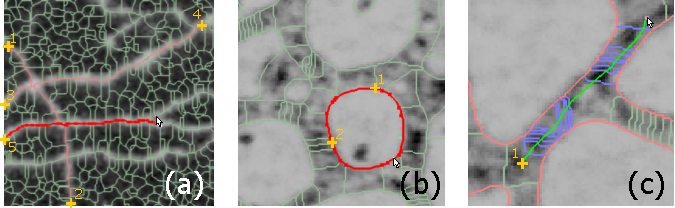
\includegraphics[width=.8\columnwidth]{figures/interactions.pdf}
    }
    \caption{Interactive tool allowing a human to specify a segmentation by labeling topological priors, specifically polylines, as opposed to individual pixels. With the shortest-path tool, a user is six clicks into labeling the foreground neurons (a). A user only needs 3 clicks to draw a closed loop (b). Finding objects crossing a free-form stroke allows rapid labeling (c). }
    \label{fig:tool}

    \vspace{-.2cm}
    
\end{figure}

%
%  Graph Heirarchies
%
\vspace{-0.4cm}
\subsection{Identifying and Labeling Topological Graph Hierarchies}
\label{Sec:labeling_hierarchies}

% % With higher persistence priors graphs leading to more expansive topological connectivity a single topological primitive in the priors subgraph may span multiple topological primitives of the same dimensionality in the priors supergraph. To accommodate this in order to best align prior subgraph labelings to that of the priors supergraph a union threshold can be provided by the user. For a given union threshold the label assigned to a priors subgraph topological primitive is assigned as the predominant class label of topological primitives within a specified percentage in the priors supergraph subset to the subgraph component. The percentage of topological priors within the priors supergraph required for assigning class labels to topological priors to which priors within the higher granularity priors graph belong is taken to be the union threshold. More formally, the class  $y_{v_j}$ of a topological prior $v_{j}$ in the priors subgraph $G_j$ subset to priors graph $G_i$, implying the persistence $p_j$ used for generating $G_j$ and persistence $p_i$ for generating $G_i$ is such that $p_j \geq p_i$, with label $y_{v_i}$ of the priors supergraph are assigned onto priors $v_{j} \subseteq v_{i}$  within the priors subgraph granted the percentage of priors of the supergraph which share the same label are above the union threshold $u$, or  such that with the given union threshold $u$ then $y_{v_j} = \ell$ if $ \dfrac{|\{ v_{i}~:~v_{i}\in v_{j}~\&~ y_{v_{i}} = \ell \}|}{|\{ v_{i}~:~v_{i}\in v_{j}\}|}\geq u$.

% \paragraph{Label Mapping of Topological Prior Super-Graph to Prior Sub-Graphs}

%With higher persistence priors graphs leading to more expansive topological connectivity a single topological primitive in the priors subgraph may span multiple topological primitives of the same dimensionality in the priors supergraph. 
A single topological primitive in a higher persistence subgraph may span multiple topological primitives in a lower persistence supergraph.  Given a labeled priors supergraph, a topological primitive in the priors subgraph is assigned the majority class label of primitives within the corresponding part of the supergraph, as long the proportion of primitives in the supergraph exceeds a user-specified percentage which we call a union threshold. 
%(Otherwise, the priors of the supergraph are not identified as components of the subgraph.)  
In this way, significant priors of the supergraph are identified as components of the subgraph.  Formally, for persistence levels $p_i$ and $p_j \geq p_i$, the class  $\ell_j$ of a topological prior $v_{p_j}$ in the priors subgraph of persistence $p_j$ is subset to priors supergraph of persistence $p_i$ with labeling scheme $\ell_i$.  Given a union threshold $u$ the label $\ell_j$ is given as follows: 
%are assigned onto priors $v_{p_j}$  within the priors subgraph such that 
%With a user-specified union threshold $u$,
$\ell_j = \ell_i$ if $ \frac{1}{|v_{p_i}~:~v_{p_i}\in~v_{p_j}|}\underset{v_{p_i} \subseteq v_{p_j}}{\sum} \bbm{1} ( \ell(v_{p_i}) = \ell_i) \geq u$. In short, each prior in the subgraph is given the predominant label of priors in the supergraph that correspond to it, so long as the majority label of priors exceeds a user-specified threshold $u$. 

